\documentclass{standalone}
\usepackage[usenames,dvipsnames]{xcolor}
\usepackage{pgfplots}

\begin{document}

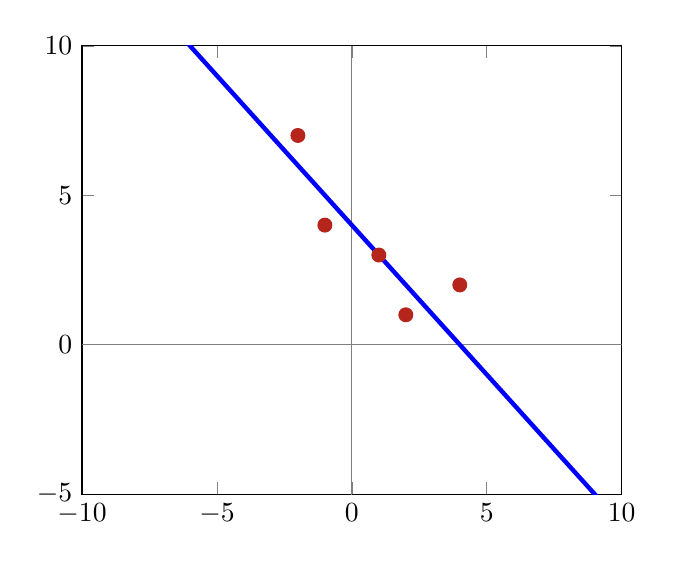
\begin{tikzpicture}
\begin{axis}[xmax=10,xmin=-10,ymax=10, ymin=-5, samples=100, title style={font=\huge}]
  \addplot[domain=-10:10, gray] (x, 0);
  \addplot[domain=-10:10, gray] (0, x);

% original error lines
  % (y_hat - y) lines - here because we want it to be behind the blue line
% (x y) -> \addplot[domain=y:2x+1, red] (x, 'x')
% (2 1) -> 
%  \addplot[domain=1:5, red] (2, x);
% (4 2) ->
%  \addplot[domain=2:9, red] (4, x);
% (-1 4) ->
%  \addplot[domain=4:-1, red] (-1, x);  
% (-2 7) ->
%  \addplot[domain=7:-3, red] (-2, x);

% new error lines
% (x y) -> \addplot[domain=y:-x+4, red] (x, 'x')
% (2 1) ->
%  \addplot[domain=1:2, red] (2, x);
% (4 2) ->
%  \addplot[domain=2:0, red] (4, x);
% (-1 4) ->
%  \addplot[domain=4:5, red] (-1, x);  
% (-2 7) ->
%  \addplot[domain=7:6, red] (-2, x);

%  \addplot[domain=-10:10, blue, ultra thick] (x, {2*x+1});
  
  \addplot[only marks, mark=*, solid, mark options={solid}, color=BrickRed, fill=BrickRed, mark size=2.5] table {
  	 1 3
  	 2 1
  	 4 2
  	 -1 4
  	 -2 7
  };




  \addplot[domain=-10:10, blue, ultra thick] (x, {-x+4});


 

\end{axis}
\end{tikzpicture}

\end{document}